%\subsection{Speicherorganisation}
%
%\subsubsection{Doubly Dynamic Linked List}\label{Appendix:Lists}
%
%In Abbildung \ref{fig:Doubly_Linked_List_2_0} wird nur der start-Pointer (head) initialisiert, ohne auf ein Element zu zeigen (NULL). Sobald der benötigte Speicherplatz des Elementes alloziiert wurde, wird der Zeiger auf die angelegte Struktur (Element) gelegt. Dem Head-Zeiger wurde nun ein Element zugewiesen und der Beginn der Liste wurde definiert.
%
%\begin{figure}[H]
%	\centering
%	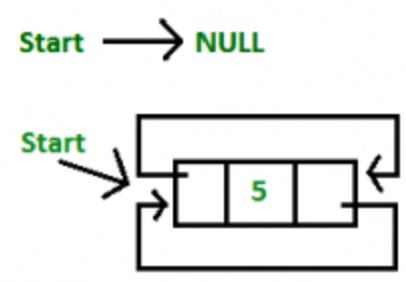
\includegraphics[width=0.5\textwidth]{graphics/Doubly_Linked_List_2_0}
%	\caption{Leerer Start-Pointer wird auf Element gerichtet, welches auf sich selber zeigt.\cite{kumar_doubly_2017}}
%	\label{fig:Doubly_Linked_List_2_0}
%\end{figure}
%
%Abbildung \ref{fig:Doubly_Linked_List_2_1} zeigt eine bestehende Liste mit zwei Elementen. Ein drittes Element soll am Schluss eingefügt werden. Dazu muss zuerst der Speicherplatz für das neue Element alloziiert werden (Data, next, prev). Danach können die Zeiger der bestehenden Elemente (in diesem Falle noch head und tail) umgelegt werden und die Zeiger des neuen Elementes auf das vorhergehende und nächste Element gelegt werden. Auch der tail-Zeiger muss nun auf das neue Element gelegt werden.
%
%\begin{figure}[H]
%	\centering
%	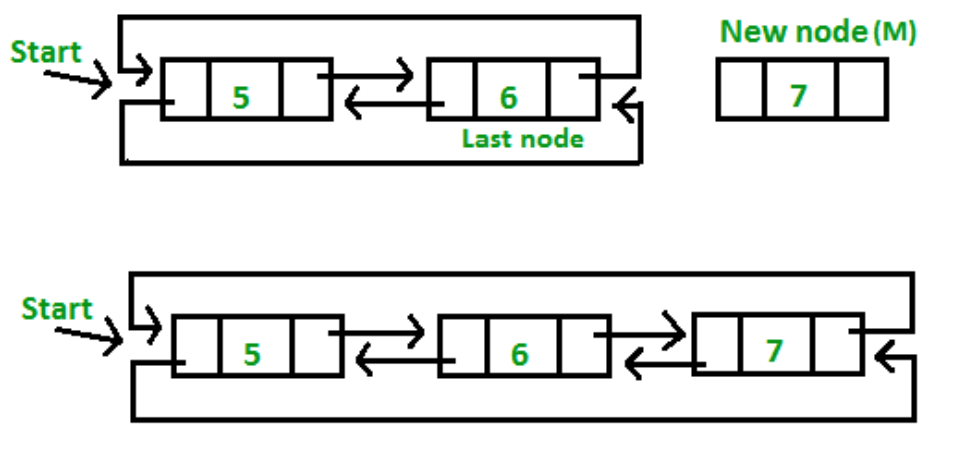
\includegraphics[width=0.5\textwidth]{graphics/Doubly_Linked_List_2_1}
%	\caption{Doppelt verkettete Liste mit zwei Elementen, woran am Ende ein neues Element hinzugefügt wird.\cite{kumar_doubly_2017}}
%	\label{fig:Doubly_Linked_List_2_1}
%\end{figure}
%
%Abbildung \ref{fig:Doubly_Linked_List_2_2} zeigt ebenfalls eine bestehende Liste mit zwei Elementen. Ein drittes Element soll am Beginn eingefügt werden. Dazu muss zuerst der Speicherplatz für das neue Element alloziiert werden (Data, next, prev). Danach können die Zeiger der bestehenden Elemente (in diesem Falle noch head und tail) umgelegt werden und die Zeiger des neuen Elementes auf das vorhergehende und nächste Element gelegt werden. Auch der head-Zeiger muss nun auf das neue Element gelegt werden.
%
%\begin{figure}[H]
%	\centering
%	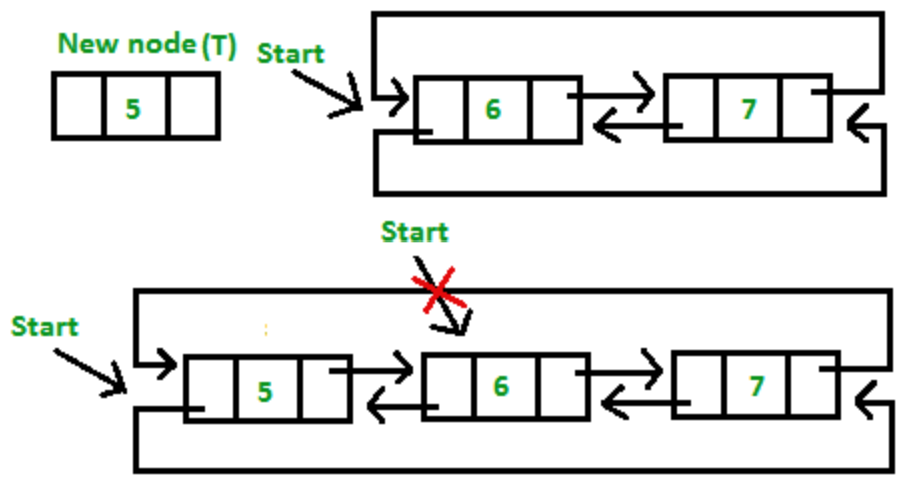
\includegraphics[width=0.5\textwidth]{graphics/Doubly_Linked_List_2_2}
%	\caption{Doppelt verkettete Liste mit zwei Elementen, woran am Anfang ein neues Element hinzugefügt wird.\cite{kumar_doubly_2017}}
%	\label{fig:Doubly_Linked_List_2_2}
%\end{figure}
%
%
%Abbildung \ref{fig:Doubly_Linked_List_2_3} zeigt eine bestehende Liste mit vier Elementen. Ein fünftes Element soll in der Mitte eingefügt werden. Dazu muss zuerst der Speicherplatz für das neue Element alloziiert werden (Data, next, prev). Danach können die Zeiger der bestehenden Elemente umgelegt werden und die Zeiger des neuen Elementes auf das vorhergehende und nächste Element gelegt werden.
%
%\begin{figure}[H]
%	\centering
%	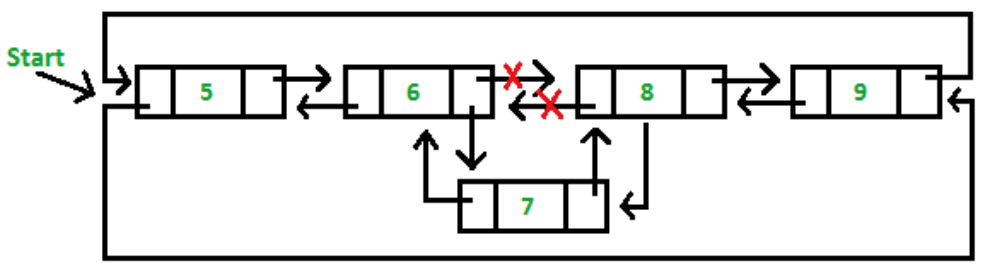
\includegraphics[width=0.5\textwidth]{graphics/Doubly_Linked_List_2_3}
%	\caption{Doppelt verkettete Liste mit vier Elementen, woran in der Mitte ein neues Element hinzugefügt wird.\cite{kumar_doubly_2017}}
%	\label{fig:Doubly_Linked_List_2_3}
%\end{figure}
%
